\documentclass[11pt]{article}

\usepackage[margin=1in]{geometry}
\usepackage[T1]{fontenc}
\usepackage{lmodern}
\usepackage{microtype}
\usepackage{amsmath}
\usepackage{graphicx}
\usepackage{booktabs}
\usepackage{array}
\usepackage{xcolor}
\usepackage{enumitem}
\usepackage{caption}
\usepackage[most]{tcolorbox}
\usepackage{titlesec}
\usepackage[hidelinks]{hyperref}

\definecolor{decisioncol}{HTML}{9A6700}
\definecolor{accentcol}{HTML}{1B5E73}
\definecolor{rulecol}{HTML}{B9C0C8}

\titleformat{\section}{\normalfont\large\bfseries\color{accentcol}}{\thesection.}{0.6em}{}
\titleformat{\subsection}{\normalfont\normalsize\bfseries}{\thesubsection}{0.6em}{}
\titlespacing*{\section}{0pt}{14pt}{6pt}
\titlespacing*{\subsection}{0pt}{10pt}{4pt}

\captionsetup{font=small,labelfont=bf,labelsep=period}
\setlist{itemsep=2pt,topsep=3pt,parsep=0pt}

\newcommand{\decflag}{{\small\textbf{\textcolor{decisioncol}{[\,decision needed\,]}}}\ }
\newcommand{\dpr}{d^{\prime}}

\hypersetup{pdftitle={Preregistration: Detecting Arithmetic Misconceptions from a Student's Written Work}}

\begin{document}

\begin{center}
{\LARGE\bfseries Preregistration}\\[6pt]
{\large Detecting Arithmetic Misconceptions from a Student's Written Work:\\[2pt]
How People Judge Explanations of Step-by-Step Solutions}\\[10pt]
{\normalsize [Author names and affiliations to be finalized]}\\[2pt]
{\small Draft compiled \today}
\end{center}

\section{Study information}\label{sec:info}

\textbf{Title.} Detecting arithmetic misconceptions from a student's written work: how people
judge whether a stated misconception explains a step-by-step solution.

\smallskip
\textbf{Authors.} [to be completed].

\smallskip
\textbf{Primary research question.} When a student's written arithmetic contains a systematic
order-of-operations misconception, how well can an observer judge whether a stated belief
(``this student thinks addition comes before multiplication'') explains the work? We ask what
makes this diagnostic judgment hard: the identity of the misconception, whether it appears
alone or together with a second one, and whether the statement matches, partially matches, or
fails to match the work. The same 240 stimuli are also judged by a Bayesian ideal observer and
by large language models, so the human results reported here are one arm of a planned
three-way comparison.

\smallskip
\textbf{Registry and timeline.} \decflag Registration venue and submission date (planned: OSF
Registries, matching the companion Numberlink registration).

\begin{tcolorbox}[colback=black!4,colframe=black!35,boxrule=0.6pt,
  left=8pt,right=8pt,top=6pt,bottom=6pt,title={\bfseries Type of registration: honesty disclosure}]
\small
This is a \emph{transparent, informed} preregistration, not a blind one. A completed pilot
($N = 24$) is reported in full in Section~\ref{sec:pilot}. The hypotheses will be written with
those results in hand and then locked; only a new confirmatory cohort
(Section~\ref{sec:power}) tests them. The 240-item stimulus pool, the trace-generating model,
and the task code are fixed before confirmatory collection begins.
\end{tcolorbox}

\section{Background and motivation}

Diagnosing \emph{why} a student got something wrong is harder than marking it wrong. Classic
work on procedural ``bugs'' in arithmetic showed that student errors are frequently systematic:
a stable, wrong rule applied consistently, rather than noise (Brown \& Burton, 1978; Brown \&
VanLehn, 1980; VanLehn, 1990). A teacher who can infer the rule from the written work can
correct the cause instead of the symptom. This inference is a signal-detection problem: given a
worked solution and a candidate explanation, decide whether the explanation actually accounts
for the steps on the page.

Our task studies that judgment in a controlled setting. The domain is order of operations
(BODMAS) in integer arithmetic, where six well-formed misconceptions can be defined exactly
(Table~\ref{tab:misconceptions}) and a generative model can simulate a learner who holds any
one or two of them. Because the stimuli come from a known generative model, ground truth is
exact, and the same inference problem can be posed to a Bayesian ideal observer that inverts
the model. The ideal observer recovers the true misconception with high reliability (for
example, its average posterior on the true rule ranges from 0.69 to 0.82 across the six
misconceptions when present alone, and it endorses category~A statements about 95\% of the
time), so the task is solvable in principle from the information on the screen. How far human
judges fall short of that ceiling, and where, is the empirical question.

\section{Methods}\label{sec:methods}

\subsection{Participants}\label{sec:participants}

Participants are recruited on Prolific and complete the task in the browser (built in the
Smile web-experiment framework). Eligibility: adults 18 or older, fluent in English, desktop
browser. A session takes about 12 minutes (pilot median 12.5, range 4.6 to 31.9). Pay is a
base rate of about \$15 per hour plus a performance bonus rising linearly from \$0 at 50\%
accuracy to \$2 at 100\% (Section~\ref{sec:measures}). One session per person. The study runs
under NYU IRB protocol IRB-FY2026-11440 (PI: Mark Ho). \decflag Confirmatory sample size and
stopping rule (Section~\ref{sec:power}). A pilot cohort ($N = 24$) collected with this task is
reported in Section~\ref{sec:pilot}.

\subsection{Materials: the misconception model and the stimulus pool}\label{sec:materials}

\textbf{The learner model.} Stimuli are generated by a model of a learner who solves integer
arithmetic expressions step by step. An expression (four operators, with brackets possible) is
represented as an evaluation DAG; an expert learner applies the conventional order of
operations, and a misconceived learner differs by holding one or two of the six misconceptions
in Table~\ref{tab:misconceptions}. Each misconception flips the validity of a local evaluation
step in both directions, so a learner with that misconception will, for example, resolve an
addition before an adjacent multiplication. Simulating a learner on an expression yields a
\emph{trace}: the sequence of intermediate expressions the student would write, one operation
at a time, ending in a final answer. Traces are screened so that every misconception the item
is said to contain actually manifests behaviorally in the written steps (the trace diverges
from the expert's), never dividing by zero and never revealing the ground truth in any
displayed field.

\begin{table}[!ht]
\centering
\small
\renewcommand{\arraystretch}{1.25}
\begin{tabular}{@{}llp{0.52\textwidth}@{}}
\toprule
\textbf{Id} & \textbf{Shorthand} & \textbf{The student believes\ldots}\\
\midrule
\texttt{add\_before\_mul} & add$<\times$ & addition should be done before multiplication\\
\texttt{add\_before\_div} & add$<\div$ & addition should be done before division\\
\texttt{sub\_before\_mul} & sub$<\times$ & subtraction should be done before multiplication\\
\texttt{sub\_before\_div} & sub$<\div$ & subtraction should be done before division\\
\texttt{same\_priority\_rtl} & RTL & equal-priority operations go right to left\\
\texttt{outside\_bracket\_first} & outside() & operations outside brackets come first\\
\bottomrule
\end{tabular}
\caption{The six order-of-operations misconceptions. A simulated learner holds one or two of
them; an expert holds none.}
\label{tab:misconceptions}
\end{table}

\smallskip
\textbf{The pool.} The stimulus pool is a fixed set of 240 items, 60 in each of four categories
(Table~\ref{tab:categories}). Every item consists of an expression, a student's step-by-step
work generated by a misconceived learner (one or two misconceptions), and a one-sentence
\emph{belief statement} attributing a specific misconception to the student (e.g., ``Isla
believes subtraction should be done before multiplication''). The named misconception either is
or is not among those that generated the trace, which fixes the item's correct answer. Each
item carries a distinct student name within a participant's session.

\begin{table}[!ht]
\centering
\small
\renewcommand{\arraystretch}{1.25}
\begin{tabular}{@{}clllc@{}}
\toprule
\textbf{Cat.} & \textbf{Misconceptions in trace} & \textbf{Statement names\ldots} & \textbf{Statement is\ldots} & \textbf{Correct answer}\\
\midrule
A & one & the one present & a full explanation & agree\\
B & one & an absent one & a foil & disagree\\
C & two & one of the two & a partial explanation & agree\\
D & two & neither & a foil & disagree\\
\bottomrule
\end{tabular}
\caption{The four stimulus categories, 60 items each. Categories A and C make ``agree'' the
correct response; B and D make ``disagree'' correct. Category C statements are true but
incomplete: the named misconception is genuinely in the work, alongside a second one the
statement does not mention.}
\label{tab:categories}
\end{table}

\begin{tcolorbox}[colback=black!3,colframe=black!30,boxrule=0.6pt,
  left=8pt,right=8pt,top=6pt,bottom=6pt,title={\bfseries Example item (category A, pool id A044)}]
\small
\textbf{Expression:}\quad $3 \div 3 + 2 - 11 \times 5$

\smallskip
\textbf{The student's work:}
\begin{quote}
$= 1 + 2 - 11 \times 5$\\
$= 1 + \,-9 \times 5$\\
$= 1 + \,-45$\\
$= -44$
\end{quote}
\textbf{Statement:}\quad ``Isla believes subtraction should be done before multiplication.''

\smallskip
The student's first step is conventional ($3 \div 3$ first), but the second step resolves
$2 - 11$ before the adjacent multiplication. The statement names exactly the misconception
that generated the work, so the correct response is to agree.
\end{tcolorbox}

\smallskip
\textbf{Category C balance.} For two-misconception items whose statement names one of the two
(category C), the pool additionally records \emph{which} of the two misconceptions is probed,
defined chronologically: whether the probed misconception's first erroneous step appears
earlier or later in the trace than its partner's. The pool balances this exactly: each of the
six misconceptions is the probed target 5 times as the early error and 5 times as the late
error. (An earlier version of the pool defined this variable by an internal canonical ordering
that was invisible to participants and confounded with misconception identity; it was
regenerated before the final pilot batch, see Section~\ref{sec:pilot-cohort}.)

\smallskip
\textbf{Answer-security audit.} Fields that would reveal the answer (category, ground-truth
misconception list, statement correctness) are never rendered. An automated audit over all 240
items verifies that the displayed expression, trace, and statement leak no ground-truth
information.

\subsection{Design and sampling}\label{sec:design}

The design is within-subject. Each participant receives 24 trials drawn from the pool: exactly
6 from each category, sampled without replacement under a rotation that spreads items evenly
across participants, with 24 distinct student names within the session. For category C the
draw is further balanced to 3 early-error and 3 late-error targets. Trial order is shuffled.
Every trial shows the expression, the student's full written work, the belief statement, and a
6-point Likert response scale (1 = Strongly Disagree, 2 = Disagree, 3 = Slightly Disagree,
4 = Slightly Agree, 5 = Agree, 6 = Strongly Agree). The same sampling code (a Python original
and a JavaScript port used by the live experiment) is archived with the registration.

\subsection{Procedure}\label{sec:procedure}

The session runs: consent form, a window-size check, task instructions, a one-question
comprehension quiz, the 24 judgment trials, a free-response feedback survey, a short
demographics form (age, gender), and a written debrief. The instructions explain that the
student's work may contain one or two consistent mistaken beliefs and that the rating should
express \emph{how well the statement explains the work shown}, explicitly not whether the
final answer is correct. The comprehension quiz asks ``What should your rating be based on?''
with four options (final-answer correctness, explanation quality, step count, handwriting);
participants must select ``How well it explains the student's work'' to proceed. In the pilot
every participant passed on the first attempt.

On each trial the response options are locked for the first 3 seconds (with a visible
countdown) to force a minimum encoding time; a trial counter (``$k$ of 24'') is shown.
Response time is measured from stimulus onset, and cursor trajectories are logged throughout
for exploratory engagement checks. There is no upper time limit.

\subsection{Measures and scoring}\label{sec:measures}

\begin{itemize}
\item \textbf{Primary: the 1--6 rating,} collapsed to a binary decision for accuracy scoring
(rating $\geq 4$ counts as ``agree''). A response is correct when the binary decision matches
the category's correct answer (Table~\ref{tab:categories}).
\item \textbf{Signal-detection quantities.} Treating ``agree'' as a yes response, categories
A/C are signal trials and B/D are noise trials: hit rate $=P(\text{agree}\mid \text{A/C})$,
false-alarm rate $=P(\text{agree}\mid \text{B/D})$, sensitivity
$\dpr = z(\text{hit}) - z(\text{FA})$ and criterion
$c = -\tfrac{1}{2}\,[\,z(\text{hit}) + z(\text{FA})\,]$ (Green \& Swets, 1966; Macmillan \&
Creelman, 2005). Rates use the $1/(2N)$ correction before $z$-scoring. This is the same
decomposition applied to the LLM arm, so the two are directly comparable.
\item \textbf{Secondary: response time} (from stimulus onset; the 3-second lock is the floor).
\item \textbf{Exploratory:} rating magnitude as graded confidence, cursor trajectories, and
the free-text feedback.
\item \textbf{Bonus.} The bonus is recomputed server-side from the raw ratings against the
answer key: $\text{bonus} = \max\!\big(0, (\text{accuracy} - 0.5)/0.5\big) \times \$2$. Chance
performance earns \$0; the graded rating scale is deliberately not incentivized so that
confidence remains an uncontaminated dependent variable.
\end{itemize}

\section{The pilot study}\label{sec:pilot}

\subsection{Cohort}\label{sec:pilot-cohort}

The pilot comprises 24 complete Prolific sessions collected in three batches (July 9, 10, and
13, 2026) of one study. All 24 sessions have 24 answered trials, a recorded bonus block,
demographics, feedback, and cursor data; all passed the comprehension quiz on the first
attempt. Category coverage is exactly balanced: 144 trials per category, 576 trials in total.
One design fix falls between batches: the first 15 participants saw the original category-C
items, in which the early/late target variable was confounded with misconception identity; the
final 9 participants saw the corrected, chronologically balanced category-C items
(Section~\ref{sec:materials}). Categories A, B, and D are identical across all 24 participants,
and the two cohorts do not differ detectably in overall performance (pooled $\dpr$ of 0.46
versus 0.59), so A/B/D analyses pool everyone, while C-specific positional analyses use only
the final 9.

Engagement was good. No trial in the entire dataset was answered within 3.5 seconds of onset
(the fastest was 4.1 s, against a 3.0 s lock), so there is no evidence of participants waiting
out the lock and clicking through. Per-participant median response times ranged from 6.4 to
47.0 seconds per trial.

\subsection{Accuracy: the task is hard, and misses are the reason}\label{sec:pilot-acc}

Overall accuracy was 0.60 (346/576), modest against the ideal observer's near-ceiling
performance on the same items. Figure~\ref{fig:overview} shows the first structure. Accuracy
on two-misconception items (0.65) exceeds one-misconception items (0.55), and the category
breakdown locates the problem: category A, where the statement names exactly the misconception
that generated the work and the correct response is to agree, sits at chance (0.49). The
foil categories B and D (0.61, 0.66) and the partial-explanation category C (0.64) are all
reliably above chance. Participants' failures are concentrated on \emph{endorsing correct
explanations}, not on rejecting wrong ones.

\begin{figure}[!ht]
\centering
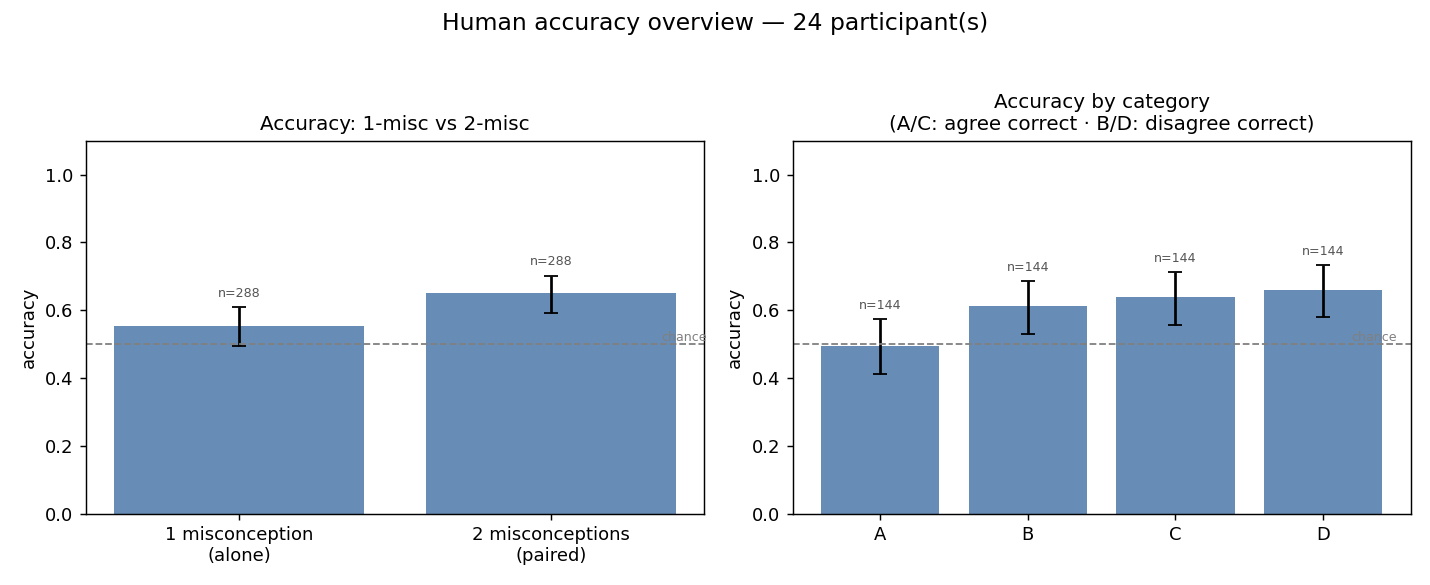
\includegraphics[width=\textwidth]{figs/accuracy_group_category.png}
\caption{Pilot accuracy ($N = 24$; 576 trials; error bars are Wilson 95\% intervals). Left:
one- versus two-misconception items. Right: the four categories. A and C require ``agree'' to
be correct; B and D require ``disagree''. Category A, the purest test of recognizing a correct
explanation, is at chance.}
\label{fig:overview}
\end{figure}

\subsection{Accuracy by misconception}\label{sec:pilot-misc}

Figure~\ref{fig:bymisc} breaks accuracy down by which misconception is present in the trace,
separately for items where it appears alone versus paired with another. Two regularities
stand out. First, the paired advantage holds for every one of the six misconceptions; it is
not driven by a single rule. Second, differences between misconceptions are modest in this
sample, with \texttt{outside\_bracket\_first} weakest when alone (0.48), which is also the
misconception the Bayesian ideal observer finds hardest. Per-misconception cells are small
(48 alone, 90 to 103 paired), so these orderings are treated as descriptive until the
confirmatory cohort.

\begin{figure}[!ht]
\centering
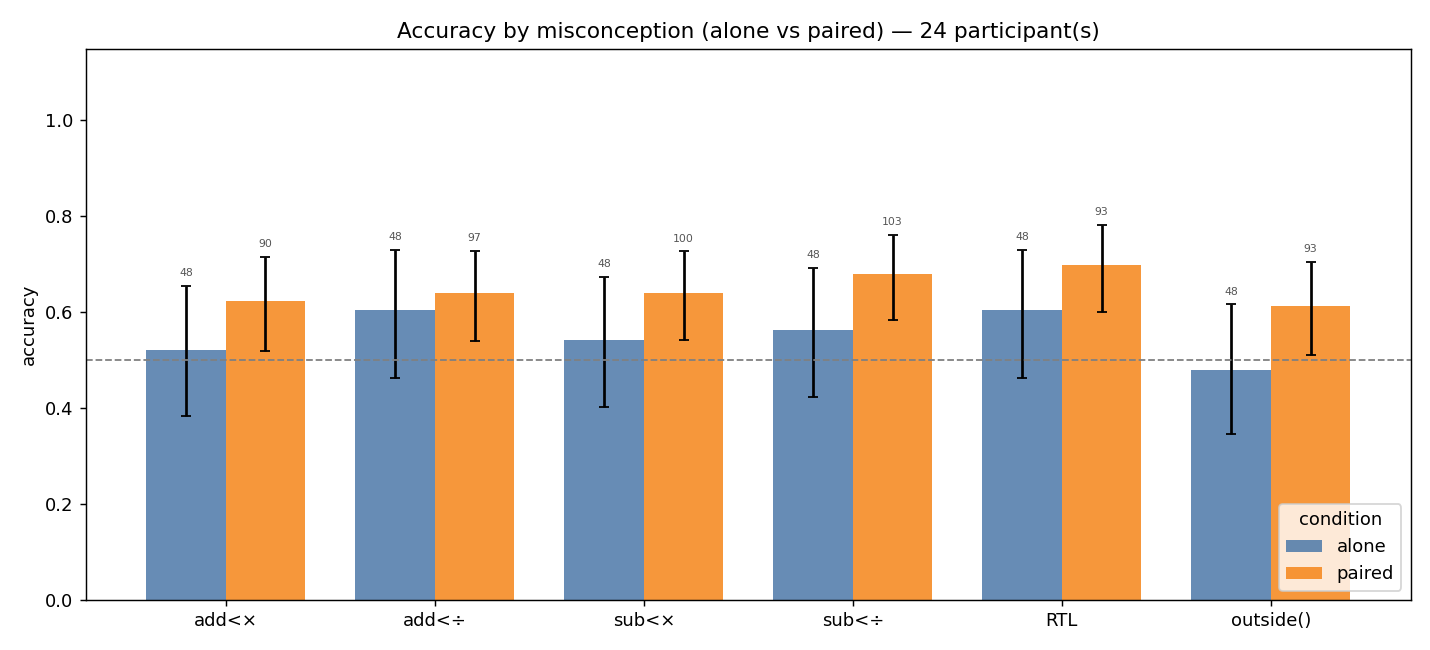
\includegraphics[width=\textwidth]{figs/accuracy_by_misconception.png}
\caption{Pilot accuracy by misconception present in the trace, alone (blue) versus paired with
a second misconception (orange). Error bars are Wilson 95\% intervals; the number above each
bar is its trial count. The paired advantage is uniform across all six misconceptions.}
\label{fig:bymisc}
\end{figure}

\subsection{Signal detection: weak average sensitivity, enormous individual spread}\label{sec:pilot-sdt}

Accuracy conflates two things: the ability to tell correct explanations from foils, and the
threshold for saying ``agree'' at all. The signal-detection decomposition of
Section~\ref{sec:measures} separates them. Pooling all trials, the hit rate was 0.57 and the
false-alarm rate 0.36, giving $\dpr = 0.51$ with a nearly neutral criterion ($c = +0.09$): on
average, participants were only weakly able to distinguish true explanations from foils, and
their chance-level category-A accuracy reflects low sensitivity rather than a blanket
reluctance to agree.

The average, however, is not a good description of anyone (Figure~\ref{fig:sdt}).
Per-participant $\dpr$ spans $-1.64$ to $+2.77$. At the top, three participants reached
$\dpr \geq 2$, and the best (92\% accuracy, $\dpr = 2.77$) outperforms every LLM regime tested
on the identical pool. In the middle, a band of participants sits between 0.4 and 1.4. At the
bottom, about seven participants are indistinguishable from chance, and two are reliably
\emph{below} it. The below-chance profiles are informative: one participant answered
``disagree'' on 23 of 24 trials (criterion $+1.73$); another spent 11 minutes on the task
(median 21.9 s per trial, never faster than 13.4 s) while answering systematically opposite to
the key ($\dpr = -1.64$), a pattern consistent with misreading the scale or judging whether
the student is mathematically correct (the answer is always no) rather than whether the
statement explains the work. Effort does not guarantee sensitivity in either direction: the
slowest participant (median 47 s per trial) landed at exactly $\dpr = 0$, and the correlation
between median response time and $\dpr$ is modest (Spearman $\rho = .39$).

\begin{figure}[!ht]
\centering
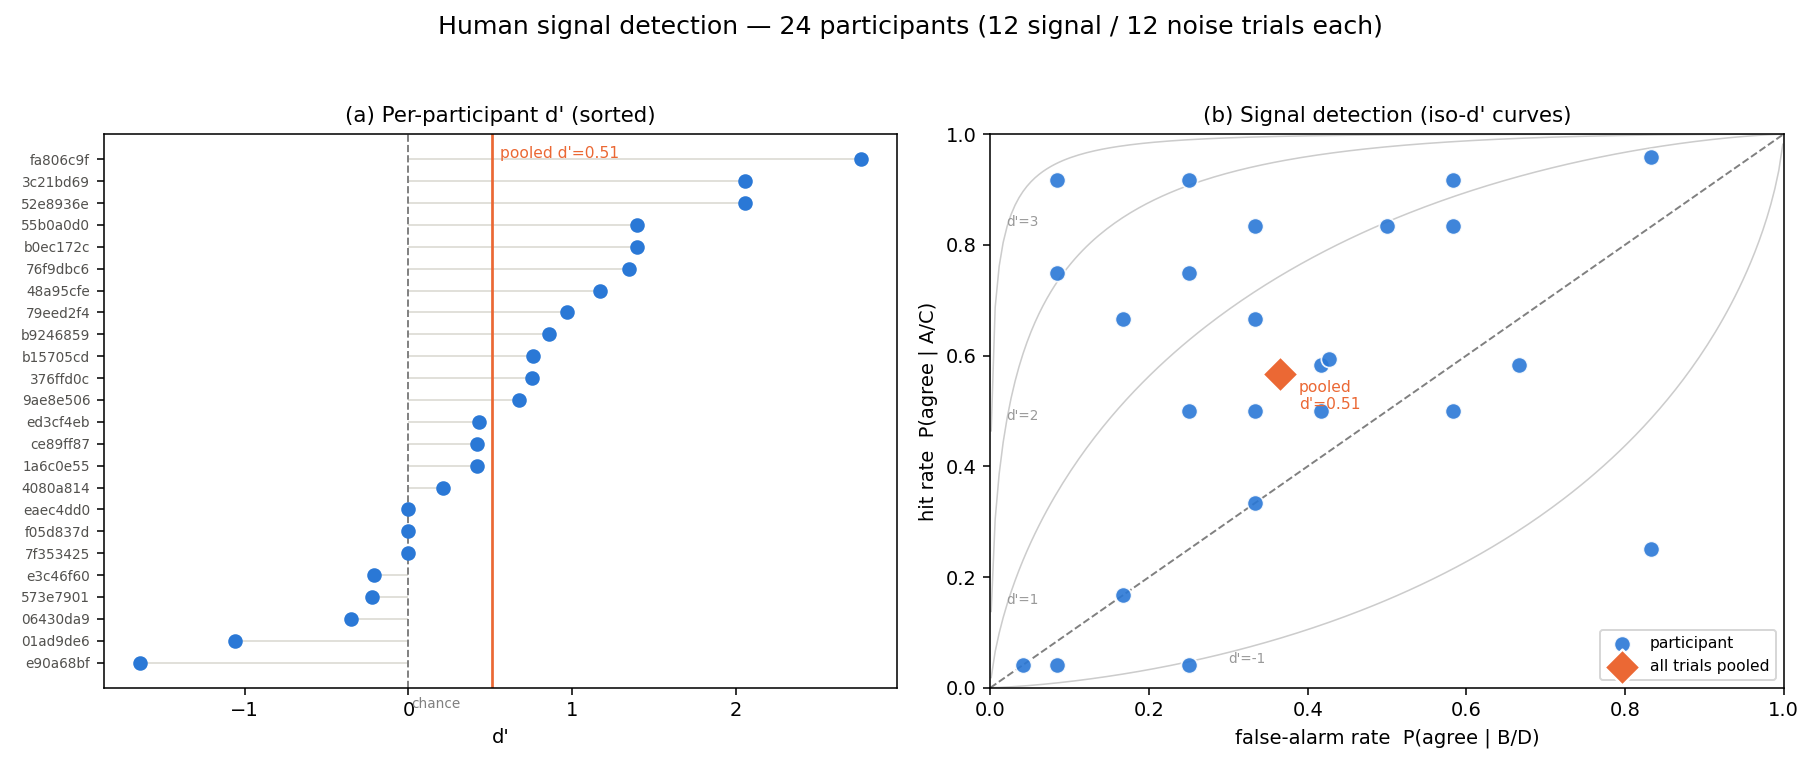
\includegraphics[width=\textwidth]{figs/human_signal_detection.png}
\caption{Pilot signal detection ($N = 24$; each participant contributes 12 signal and 12 noise
trials). Left: per-participant $\dpr$, sorted; the orange line marks the pooled value. Right:
each participant in ROC space against iso-$\dpr$ curves; the diamond is the pooled point.
Points below the diagonal are participants who reversed the mapping between evidence and
response. The spread, from $-1.64$ to $+2.77$, is the pilot's clearest single result.}
\label{fig:sdt}
\end{figure}

\subsection{What the pilot fixes for the confirmatory study}\label{sec:pilot-lessons}

Three lessons carry forward. (1)~The task produces genuine individual differences, so
participant-level exclusion rules must be set in advance; a response-time rule would exclude
almost no one (Section~\ref{sec:excl}). (2)~Category A at chance alongside above-chance B, C,
and D is the central phenomenon a confirmatory cohort must probe; hypotheses will be locked
around it. (3)~The corrected category-C items arrived only for the final batch, so positional
(early/late) questions about partial explanations have 9 usable participants (agree rate 0.63
on early-error targets versus 0.56 on late; far from decisive) and need the confirmatory
sample.

\section{Research questions and candidate hypotheses}\label{sec:hyp}

\decflag The hypotheses below are candidates drafted from the pilot; they are to be discussed,
finalized, and locked before confirmatory collection. Directionality, test families, and
correction procedures will be fixed at that point.

\begin{itemize}
\item \textbf{H1 (recognition deficit).} Accuracy on match items (A) is lower than on foil
items (B). Pilot: 0.49 versus 0.61. Equivalent framing: sensitivity to correct explanations
is the binding constraint, not response bias.
\item \textbf{H2 (partial explanations).} Do people penalize or reward incompleteness? Mean
rating on C versus A. Pilot: C is rated \emph{higher} than A (3.97 versus 3.48), the opposite
of the LLM-with-reasoning pattern on the same pool; direction to be registered as a two-sided
question.
\item \textbf{H3 (difficulty ordering).} Per-misconception human accuracy correlates with the
Bayesian ideal observer's per-misconception marginals (hardest: \texttt{outside\_bracket\_first};
easiest: \texttt{same\_priority\_rtl}).
\item \textbf{H4 (positional effect in partial explanations).} In category C, agreement is
higher when the probed misconception's error appears earlier in the trace. Pilot (usable
cohort only): 0.63 versus 0.56.
\end{itemize}

\section{Analysis plan (skeleton)}\label{sec:analysis}

\decflag To be completed once hypotheses are locked. The intended shape, mirroring the
companion registration: one logistic mixed-effects model for trial-level accuracy with planned
category contrasts and by-participant and by-item random effects; a parallel model for the
graded rating; signal-detection indices computed per participant; Holm correction within test
families; estimates always reported with 95\% confidence intervals.

\subsection{Exclusions (candidate rules)}\label{sec:excl}

\textbf{Trial level.} The 3-second lock makes fast-guess trials impossible by construction
(pilot minimum 4.1 s); an upper cutoff (e.g., 120 s) \decflag is to be set from the pilot
response-time distribution.

\smallskip
\textbf{Participant level.} Exclude sessions that are incomplete, unmatched to a valid
Prolific identifier, or from a repeated identifier. \decflag The open decision is a
performance gate. The pilot shows the case for one: two participants were reliably below
chance (consistent with reversed scale use), and their trials actively mislead any pooled
analysis. A candidate rule is binomial: exclude participants whose accuracy is significantly
\emph{below} chance (at most 7 of 24 correct, one-sided $p < .05$), which removes reversers
while keeping honest chance-level performers; analyses would additionally be reported with no
gate as a sensitivity check. Alternatives: no gate (the companion registration's choice), or
a symmetric above-chance requirement (which would have excluded roughly a third of the pilot
and changes the population being described).

\subsection{Sample size}\label{sec:power}

\decflag To be computed from the pilot once hypotheses are locked, following the companion
registration's method: per-participant effect sizes for each planned contrast, powered at
90\% at the worst-case Holm threshold. The pilot's individual-difference spread suggests the
binding constraint will be between-participant variance in $\dpr$, not trial counts.

\section{Reproducibility and materials}\label{sec:repro}

The 240-item pool (\texttt{stimulus\_pool.json}) is the canonical stimulus artifact and is
byte-identical between the generating repository and the deployed experiment. The learner
model, pool generator, sampling code (Python and the deployed JavaScript port), the Bayesian
ideal observer, and the LLM experiment pipeline are in the same repository and are archived
with the registration. Anonymized trial-level data and analysis code will be shared at the
registry when the manuscript is submitted. Deviations from the locked plan will be reported in
a labeled deviations section.

\section{Decisions to resolve before registration}\label{sec:decisions}

\begin{tcolorbox}[colback=decisioncol!5,colframe=decisioncol!55,boxrule=0.8pt,
  left=10pt,right=10pt,top=8pt,bottom=8pt]
\small
\begin{enumerate}[leftmargin=1.5em,label=\arabic*.]
\item \textbf{Hypotheses (Section~\ref{sec:hyp}).} Finalize the set, directions, and test
families; decide whether the LLM and ideal-observer comparisons are registered here or in a
companion document.
\item \textbf{Performance gate (Section~\ref{sec:excl}).} Choose among below-chance exclusion
(candidate), no gate, or an above-chance requirement.
\item \textbf{Sample size (Section~\ref{sec:power}).} Run the power analysis and set the
minimum $N$ and stopping rule.
\item \textbf{Old-pool category-C trials (Section~\ref{sec:pilot-cohort}).} Confirm they are
excluded from all C-specific confirmatory analyses (recommended) or retained descriptively.
\item \textbf{Trial-level upper response-time cutoff (Section~\ref{sec:excl}).}
\item \textbf{Registry and timeline (Section~\ref{sec:info}).}
\item \textbf{Authorship (Section~\ref{sec:info}).}
\end{enumerate}
\end{tcolorbox}

\section*{References}
\addcontentsline{toc}{section}{References}
{\setlength{\parindent}{-1.6em}\leftskip=1.6em\small

Brown, J. S., \& Burton, R. R. (1978). Diagnostic models for procedural bugs in basic
mathematical skills. \textit{Cognitive Science, 2}(2), 155--192.\par\smallskip

Brown, J. S., \& VanLehn, K. (1980). Repair theory: A generative theory of bugs in procedural
skills. \textit{Cognitive Science, 4}(4), 379--426.\par\smallskip

Green, D. M., \& Swets, J. A. (1966). \textit{Signal detection theory and psychophysics}.
Wiley.\par\smallskip

Macmillan, N. A., \& Creelman, C. D. (2005). \textit{Detection theory: A user's guide} (2nd
ed.). Lawrence Erlbaum Associates.\par\smallskip

VanLehn, K. (1990). \textit{Mind bugs: The origins of procedural misconceptions}. MIT
Press.\par

}

\end{document}
